51. \begin{figure}[ht!]
\center{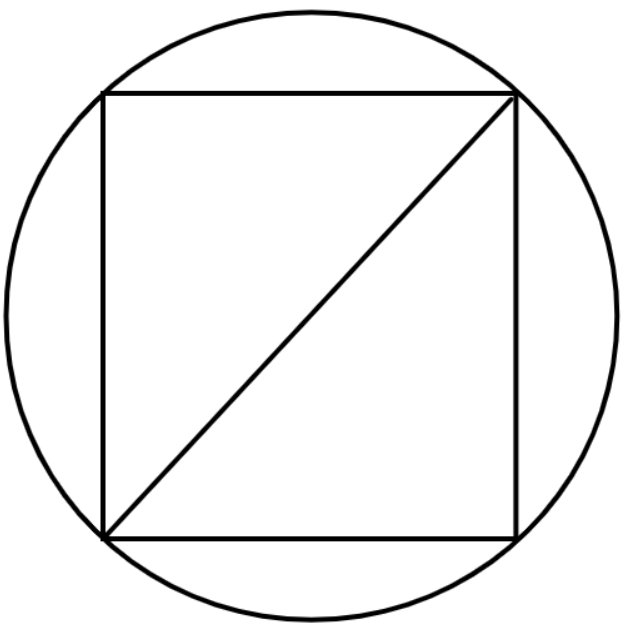
\includegraphics[scale=0.35]{g9-51.png}}
\end{figure}\\
Так как прямой угол опирается на диаметр, диагональ квадрата равна диаметру окружности, а значит она равна $2\cdot\sqrt{12}=4\sqrt{3}.$ Углы равностороннего треугольника равны по $60^\circ,$ найдём радиус искомой окружности по теореме синусов: $\cfrac{4\sqrt{3}}{\sin(60^\circ)}=2R,\ R=4.$\newpage\noindent
